\documentclass[12pt, a4paper, twocolumn]{article}

% Packages
\usepackage{graphicx} %  images
\usepackage{amsmath} % equations
\usepackage[left=1.5cm, right=1.5cm, top=1.785cm, bottom=2.0cm]{geometry}

\newcommand\blfootnote[1]{%
  \begingroup
  \renewcommand\thefootnote{}\footnote{#1}%
  \addtocounter{footnote}{-1}%
  \endgroup
}

% Document information
\title{Title here}
\author{Author here,\ddag\textit{$^{\ast a}$}}
\date{}
\begin{document}

\twocolumn[  \begin{@twocolumnfalse}    \maketitle    \begin{abstract}      Abstart here. \end{abstract}  \end{@twocolumnfalse}]


\blfootnote{\textit{$^{a}$~ note here}}

\blfootnote{\ddag~and here}

% Introduction
\section{Introduction}
testestest

\begin{figure}[h]
  \centering
    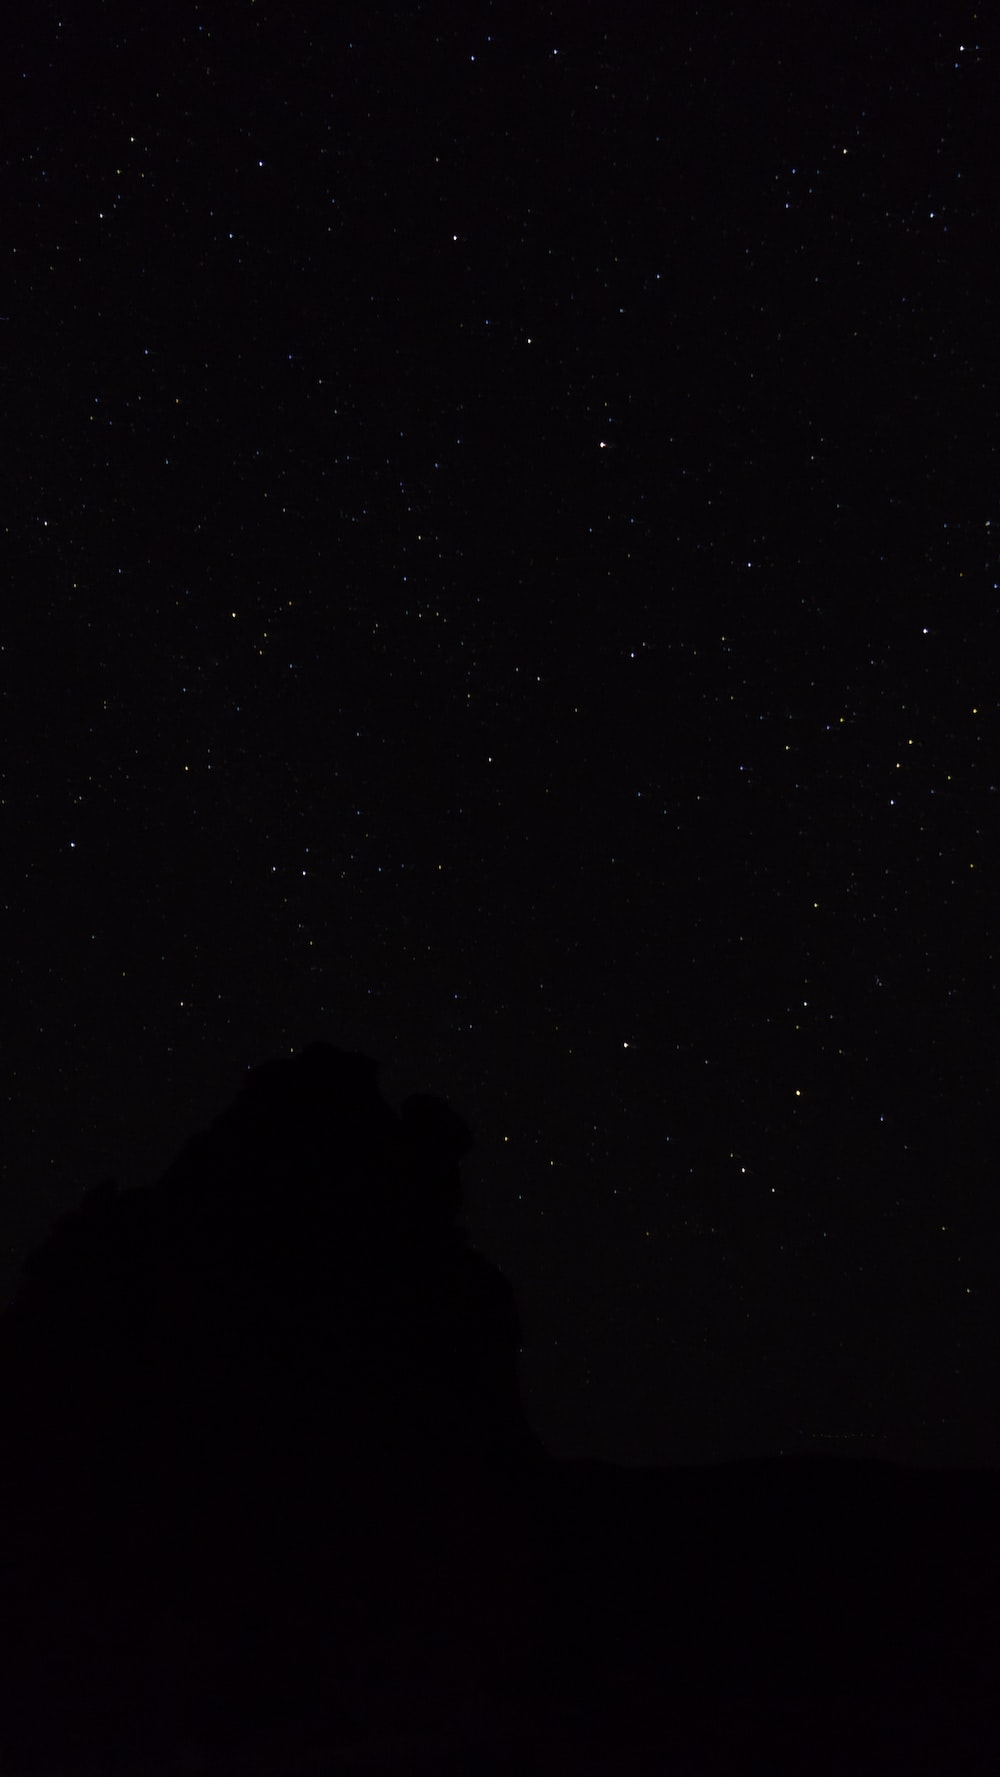
\includegraphics[width=\textwidth]{test.png}
    \caption{(a) caption here }
    \label{fig1}
  \end{figure}

%If notes are included in your references you can change the title from 'References' to 'Notes and references' using the following command:
\renewcommand\refname{References}

%%%REFERENCES%%%
\bibliographystyle{unsrt} 
\bibliography{thebibliography} %You need to replace "rsc" on this line with the name of your .bib file
% \bibliographystyle{rsc} %the RSC's .bst file

\end{document}
